
\documentclass[border=0pt]{standalone}
\usepackage{graphicx}
\usepackage{fancyvrb}
\usepackage{xcolor}
\usepackage{bm}
\usepackage{pgf}
\usepackage{tikz}
\usepackage[vlined,algoruled,linesnumbered]{algorithm2e}


\definecolor{myGray}{rgb}{0.85,0.85,0.85}

\begin{document}

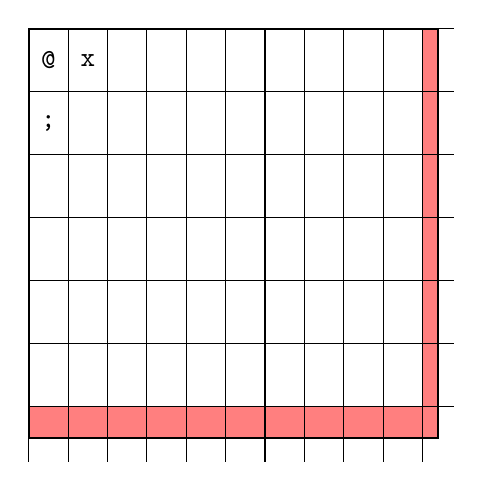
\begin{tikzpicture}
    \draw[fill=red,opacity=0.5] (5,0) rectangle (5.2,-5.2);
    \draw[fill=red,opacity=0.5] (0,-4.8) rectangle (5,-5.2);
    \draw[xstep=0.5,ystep=0.8] (0,0) grid (5.4,-5.5); 
    \draw[thick] (0,0) rectangle (5.2,-5.2);
    \node at (0.25, -0.4) {\Verb|@|};
    \node at (0.75, -0.4) {\Verb|x|};
    \node at (0.25, -1.2) {\Verb|;|};
\end{tikzpicture}


\end{document}
